\documentclass[11pt,a4paper]{article}
\usepackage{fontspec}
\setmainfont{Latin Modern Roman}
\newfontfamily\cjkfont{Noto Serif SC}
\newfontfamily\coverfont{Times New Roman}
\usepackage{microtype}
\usepackage{geometry}
\geometry{margin=27mm}
\usepackage{amsmath,amssymb}
\usepackage{booktabs}
\usepackage{array}
\usepackage{graphicx}
\usepackage{caption}
\usepackage{subcaption}
\usepackage{float}
\usepackage{xcolor}
\usepackage{enumitem}
\usepackage{tikz}
\usetikzlibrary{arrows.meta,positioning,fit,calc}
\usepackage{hyperref}
\hypersetup{colorlinks=true,linkcolor=blue!50!black,citecolor=blue!50!black,urlcolor=blue!50!black}

\newcommand{\method}[1]{\textsc{#1}}
\postdisplaypenalty=10000
\clubpenalty=10000
\widowpenalty=10000

\begin{document}
% Cover coordinates match the supplied Word template in PDF points on A4.
\begin{titlepage}
\thispagestyle{empty}
\begin{tikzpicture}[remember picture,overlay,x=1bp,y=-1bp]
\begin{scope}[shift={(current page.north west)}]
  \draw[line width=0.5bp] (373.6,99.1) rectangle (524.4,196.7);
  \draw[line width=0.5bp] (441.6,99.1) -- (441.6,196.7);
  \draw[line width=0.5bp] (373.6,147.9) -- (524.4,147.9);
  \node[anchor=north,inner sep=0,font=\coverfont\bfseries\fontsize{14}{17}\selectfont]
       at (407.6,101) {Score:};
  \node[anchor=north,inner sep=0,font=\coverfont\bfseries\fontsize{14}{17}\selectfont]
       at (407.6,150) {Grader:};
  \node[anchor=north,inner sep=0] at (297.66,196.94)
       {
\includegraphics[width=194.7bp,height=52.4bp]{figures/university_wordmark.png}};
  \node[anchor=north,inner sep=0,font=\coverfont\bfseries\fontsize{22}{27}\selectfont\addfontfeatures{LetterSpace=9.09}]
       at (297.66,251) {Machine Learning II Course Report};
  \node[anchor=north west,inner sep=0,font=\coverfont\bfseries\fontsize{15}{18}\selectfont]
       at (161.3,311) {Title:};
  \node[anchor=north west,inner sep=0,text width=299bp,
        font=\coverfont\bfseries\fontsize{14}{19}\selectfont,align=left]
       at (211,310) {Debugging the Black Box:\\
         Explainable Interventions for RL\\
         and MPC Portfolio Control};
  \node[anchor=north west,inner sep=0,font=\coverfont\bfseries\fontsize{12}{15}\selectfont]
       at (165.5,378) {Student ID:};
  \node[anchor=north west,inner sep=0,font=\coverfont\fontsize{12}{15}\selectfont]
       at (230,378) {\underline{\makebox[147bp][l]{I202680256}}};
  \node[anchor=north west,inner sep=0,font=\coverfont\bfseries\fontsize{12}{15}\selectfont]
       at (165.5,410.5) {Name:};
  \node[anchor=north west,inner sep=0,font=\coverfont\fontsize{12}{15}\selectfont]
       at (207,410.5) {\underline{\makebox[200bp][l]{Ivan Pavliuk {\cjkfont 林伟}}}};
  \node[anchor=north west,inner sep=0,font=\coverfont\bfseries\fontsize{12}{15}\selectfont]
       at (165.5,443) {Major:};
  \node[anchor=north west,inner sep=0,font=\coverfont\fontsize{12}{15}\selectfont]
       at (207,443) {\underline{\makebox[267bp][l]{Big Data and Machine Learning}}};
  \node[anchor=north west,inner sep=0,font=\coverfont\bfseries\fontsize{12}{15}\selectfont]
       at (165.5,475.5) {Course Instructors:};
  \node[anchor=north west,inner sep=0,font=\coverfont\fontsize{12}{15}\selectfont]
       at (274,475.5) {\underline{\makebox[200bp][l]{{\cjkfont 朱力军，万一鸣}}}};
  \node[anchor=north west,inner sep=0,font=\coverfont\bfseries\fontsize{12}{15}\selectfont]
       at (165.5,508) {School / Department / Institute:};
  \node[anchor=north west,inner sep=0,text width=310bp,align=left,
        font=\coverfont\fontsize{12}{17}\selectfont]
       at (165.5,530) {\underline{School of Artificial Intelligence and Innovation}};
  \node[anchor=north,inner sep=0,font=\coverfont\bfseries\fontsize{14}{17}\selectfont]
       at (297.66,580) {Month 11, Day 24, 2026};
\end{scope}
\end{tikzpicture}
\null
\end{titlepage}

\pagenumbering{arabic}

\begin{abstract}
This project report compares a tabular reinforcement-learning portfolio controller with a transparent receding-horizon model-predictive controller on a real US market stress panel. The dataset contains market and macro series; the tabular RL state uses SPY trend, VIX percentile, and HYG--LQD relative performance. The RL controller is trained on 2010--2017 data. A validation period from 2018--2021 selects one primitive intervention, while the frozen test from 2022-01-03 to 2023-02-28 is used for the historical before--after comparison. On the frozen test, baseline RL has Sharpe $-0.653$ and maximum drawdown $-21.71\%$; baseline MPC has Sharpe $0.322$ and maximum drawdown $-6.62\%$. A train-only behavior vocabulary identifies a stress-overexposure primitive. Mapping it to cash preservation improves RL to Sharpe $-0.460$ and maximum drawdown $-14.95\%$, with a control-adjusted Sharpe lift of $+0.214$ against twenty matched-random repairs. Robust MPC reaches Sharpe $1.990$ on the exploratory 2023--2026 outer holdout with maximum drawdown $-7.44\%$. The results support explainability as a debugging and control interface, while the outer holdout also shows that a local RL repair is not a universal improvement.
\end{abstract}

\paragraph{Keywords:} reinforcement learning; model predictive control; explainable AI; self-supervised learning; portfolio control; stress regime; counterfactual intervention.

\section{Introduction}
Financial decisions are sequential, costly, and exposed to distribution shift. A controller can look strong in a calm period and fail when volatility and credit conditions change. This makes explainability a validation problem rather than a presentation feature. The useful question is whether an explanation identifies a behavior that can be edited under a frozen policy and whether the edit survives controls.

This study compares two methods taught in machine learning courses. Reinforcement learning (RL) adapts through a value function and can represent long-run consequences. Model predictive control (MPC) repeatedly solves an explicit optimization problem and exposes its trade-offs in the objective and constraints. The comparison is therefore also a comparison of two explanation regimes: a discrete behavior vocabulary for RL and an explicit objective for MPC.

The experiment follows three stages. Stage A measures both controllers before any intervention. Stage B discovers behavior primitives, labels their market mechanisms, and selects one low-dose repair on validation data. Stage C repeats the frozen-test comparison and evaluates matched-random and opposite-direction controls. The central claim is deliberately narrow: a useful explanation should identify an editable behavior and make a controlled change whose effect is larger than an equally sized arbitrary edit.

\section{Problem Formulation}
\subsection{Sequential portfolio decision problem}
The portfolio controller uses an approximate discrete market state. At day $t$, $s_t$ combines SPY trend, VIX percentile, and a credit-relative-return flag; previous allocation is tracked separately for turnover, not included in the 18-state Q-table. The action $a_t$ is one of six allocations over SPY, TLT, HYG, and residual cash. The RL action is applied to the return from $t$ to $t+1$. Its daily learning reward is
\begin{equation}
r_t = \log\!\left(1+w(a_t)^\top R_{t+1}\right) - \lambda_{\mathrm{turn}}\left\|w(a_t)-w(a_{t-1})\right\|_1,
\qquad \lambda_{\mathrm{turn}}=0.0006.
\label{eq:rl-reward}
\end{equation}
The reward values subsequent growth and subtracts a penalty for trading.
Here $t$ is the decision index, $s_t$ its observed market state, and $a_t$ the chosen action identifier. The column vector $w(a_t)$ gives three risky-asset weights; $w(a_{t-1})$ is the previous target. The vector $R_{t+1}$ contains asset returns realized after the RL decision. The transpose $\top$ makes their dot product a scalar portfolio return. The scalar 1 represents starting wealth, $\log$ is the natural logarithm, and $\|\cdot\|_1$ adds the absolute changes of risky weights. The coefficient $\lambda_{\mathrm{turn}}=0.0006$ is six basis points per unit of turnover, identical to $c$ below. Thus $r_t$ is a shaped learning reward, not the gross return plotted later. The policy cannot observe $R_{t+1}$ at selection time; chronology and the different MPC indexing are specified in the methods.

\subsection{Receding-horizon MPC}
MPC uses the same action grid. Its original baseline estimates daily mean $\mu_t$ from the previous twenty observations and covariance $\Sigma_t$ from the previous sixty, then scores a horizon $H=5$:
\begin{equation}
J_t(w) = H w^\top\mu_t - \lambda_{\Sigma}H w^\top\Sigma_t w - \lambda_{\mathrm{turn}}\left\|w-w_{t-1}\right\|_1,
\qquad \lambda_{\Sigma}=8.
\label{eq:mpc-objective}
\end{equation}
MPC ranks a candidate by forecast gain minus variance and turnover penalties.
Here $J_t(w)$ is a scalar score for candidate weight vector $w$ at row $t$, not money earned. $H$ is the number of forecast days; $w^\top\mu_t$ is the predicted daily portfolio return, and $w^\top\Sigma_t w$ its daily variance including cross-asset covariance. Risk coefficient $\lambda_\Sigma=8$ scales the variance penalty and is denoted $\lambda$ below. The previous target is $w_{t-1}$; $\lambda_{\mathrm{turn}}\|w-w_{t-1}\|_1$ penalizes its change. This approximation holds one candidate constant over the horizon. The state-dependent variant adds a SPY-weight cap and a separate VIX penalty; its full equation is given below.

\section{Methods and Algorithms}
\subsection{RL challenger and MPC baselines}
The RL challenger is tabular Q-learning over 18 stress states formed by three SPY trend bins, three VIX-percentile bins, and a credit-relative-return flag. Six actions range from cash preservation to full SPY exposure. The Q-table is updated for 160 passes through the training period with epsilon-greedy exploration, discount factor $0.985$, and learning rate $0.08$. The MPC baseline uses rolling sample moments; robust MPC adds the explicit stress constraint.

\subsection{Detailed mathematical specification of the controllers}
The six controllers are RL baseline, RL repaired, baseline MPC, state-dependent MPC, ensemble MPC, and minimax MPC. All use the same six allocations. Action identifiers are labels: action 5 is not more aggressive than action 4.

\paragraph{Common symbols and action grid.}
The index $t$ labels a trading observation; $i$ labels an asset and $j$ a historical observation. There are $n=3$ risky assets, ordered as SPY, TLT, HYG. The action set is $\mathcal A=\{0,1,2,3,4,5\}$. The column vector $w(a)\in\mathbb R^3$ contains the three target wealth fractions for action $a$, with components $w_i(a)$. Cash is residual:
\begin{equation}
w_{\mathrm{cash}}(a)=1-\mathbf1^\top w(a),\qquad \mathbf1=(1,1,1)^\top.
\label{eq:cash-weight}
\end{equation}
The share not assigned to the three risky assets stays in cash.
Here $\mathbf1$ is a vector of ones, $\top$ is transpose, and $\mathbf1^\top w$ adds the risky weights; the scalar 1 denotes 100\% of wealth. Cash earns zero interest in the simulation. Superscripts naming controllers or windows are labels, not powers.

\begin{table}[H]
\centering
\caption{Six candidate portfolios; weights are fractions of wealth.}
\label{tab:action-grid}
\begin{tabular}{@{}rlrrrr@{}}
\toprule
Action & Allocation & SPY & TLT & HYG & Cash\\
\midrule
0 & Cash & 0 & 0 & 0 & 1\\
1 & Defensive & 0.25 & 0.50 & 0.25 & 0\\
2 & Balanced & 0.50 & 0.25 & 0.25 & 0\\
3 & Growth & 0.75 & 0.125 & 0.125 & 0\\
4 & Equity & 1 & 0 & 0 & 0\\
5 & Equity and bonds & 0.50 & 0.50 & 0 & 0\\
\bottomrule
\end{tabular}
\end{table}
Each decision selects a row of this table rather than a continuous weight vector.

\paragraph{Return, turnover, and chronology.}
The adjusted price of asset $i$ on observation $t$ is $P_{i,t}$; its simple return is $R_{i,t}=P_{i,t}/P_{i,t-1}-1$. The column vector $R_t$ collects the three asset returns ending at $t$.
\begin{equation}
\begin{aligned}
g_{t+1}(a_t)&=w(a_t)^\top R_{t+1}=\sum_{i=1}^{3}w_i(a_t)R_{i,t+1},\\
\tau_t&=\|w(a_t)-w(a_{t-1})\|_1
       =\sum_{i=1}^{3}|w_i(a_t)-w_i(a_{t-1})|.
\end{aligned}
\label{eq:return-turnover}
\end{equation}
The return is a weighted sum of asset returns, while turnover adds the sizes of the trades.
Here $a_t$ is the selected action and $a_{t-1}$ is the previous action. The scalar $g_{t+1}$ is the subsequent simple portfolio return. The summation sign $\sum$ adds three contributions. The transpose makes a dot product, giving a scalar. Absolute-value bars count purchases and sales positively; $\|\cdot\|_1$ is the sum of these absolute changes. The saved implementation uses successive target weights, not weights drifted by asset returns, and excludes cash from turnover.

RL features at row $t$ select an action credited with row $t+1$'s return. MPC moment estimates use rows strictly before $t$ and receive row $t$'s return. The state-dependent MPC gate additionally reads row-$t$ stress features while receiving row-$t$ returns: its saved output is not a fully lagged executable backtest. This revision preserves the stored outputs and explains their actual calculation. Their historical evaluation windows have already been inspected, so repeated analysis does not create an independent test.

\paragraph{RL baseline and learning reward.}
\begin{equation}
\begin{aligned}
a_t^{\mathrm{RL}}&=\arg\max_{a\in\mathcal A}Q(s_t,a),\\
r_t&=\log(1+g_{t+1}(a_t^{\mathrm{RL}}))-c\tau_t,\qquad c=0.0006.
\end{aligned}
\label{eq:rl-detailed}
\end{equation}
The table selects an action and learning balances subsequent growth against turnover.
The state $s_t$ is one of 18 bins of SPY trend, VIX percentile, and credit-relative return. $Q(s_t,a)$ is an estimate of discounted reward for that state-action pair. $\arg\max$ returns an action identifier, whereas $\max$ returns the score itself; ties choose the first grid entry. $r_t$ is a learning reward, distinct from simple return $g_{t+1}$. $\log$ is the natural logarithm and $1+g_{t+1}$ is the gross wealth multiplier. The coefficient $c$ is six basis points per unit of risky-weight turnover; $c\tau_t$ is a penalty. The code floors the logarithm's argument at $10^{-8}$ for numerical protection.

\begin{equation}
Q(s_t,a_t)\leftarrow Q(s_t,a_t)+
\eta\left[r_t+\gamma_d\max_{a'\in\mathcal A}Q(s_{t+1},a')-Q(s_t,a_t)\right].
\label{eq:q-update-detailed}
\end{equation}
Q-learning adjusts its old estimate toward the observed reward plus a continuation estimate.
The assignment arrow $\leftarrow$ denotes an update. $\eta=0.08$ is its step size. The bracketed temporal-difference error consists of observed reward, discounted best next-state value, and subtraction of the old estimate. The index $a'$ ranges over possible next actions and $s_{t+1}$ is the next state. The discount factor $\gamma_d=0.985$ weights future rewards and is unrelated to MPC risk aversion $\lambda$. The table starts at zero and trains for 160 passes; exploration decreases from 0.21 to approximately 0.011. Evaluation uses greedy actions and does not update $Q$.

\begin{equation}
W_T=W_0\prod_{t=0}^{T-1}(1+g_{t+1}),\qquad
\log(W_T/W_0)=\sum_{t=0}^{T-1}\log(1+g_{t+1}).
\label{eq:compounding}
\end{equation}
Wealth compounds by multiplication; logs express that same growth as a sum.
$W_0$ is initial wealth, $W_T$ is terminal wealth after $T$ return intervals, and $\prod$ multiplies their wealth factors. This gross accounting identity assumes no external cash flows. It concerns undiscounted log returns; a discounted sum of penalized rewards is not exactly log terminal wealth. A 50\% loss followed by a 50\% gain leaves $0.5\times1.5=0.75$ of starting wealth. A logarithm neither creates compounding nor imposes a maximum-drawdown constraint.

\paragraph{RL repair and primitive assignment.}
\begin{equation}
\hat z_t=\arg\min_{k\in\{0,\ldots,K-1\}}\|S(\phi_t)-b_k\|_2^2,\qquad K=6.
\label{eq:primitive-detailed}
\end{equation}
The behavior descriptor receives the label of its nearest training centroid.
The vector $\phi_t$ contains state code, original action code, stress flag, twenty-day SPY return, VIX percentile, and twenty-day HYG-minus-LQD return. $S$ standardizes features using training means and standard deviations. $b_k$ is standardized KMeans centroid $k$; $K$ is the number of centroids. The squared Euclidean norm $\|\cdot\|_2^2$ sums squared component differences. $\arg\min$ returns the closest identifier; the hat in $\hat z_t$ denotes an inferred label. Scaler and centroids are frozen after training.

\begin{equation}
a_t^{\mathrm{rep}}=
\begin{cases}
0,&\hat z_t=0,\\
a_t^{\mathrm{RL}},&\hat z_t\ne0.
\end{cases}
\label{eq:repair-detailed}
\end{equation}
Only primitive 0 activates the cash substitution; all other decisions keep their baseline actions.
The superscript $\mathrm{rep}$ denotes the executed repaired action. The two zeros have different roles: primitive identifier 0 triggers the rule, while action identifier 0 selects cash. Classification uses the unedited baseline descriptor, not repeated reclassification of the edited action. The mapping is selected using validation and leaves $Q$ unchanged. The saved trajectory field \texttt{ret} is a gross simple return; the turnover penalty affects training but is not deducted from this field.

\paragraph{Rolling moments.}
Let $L$ denote the desired memory length and $N_{t,L}$ the available number of historical rows, capped at $L$. The saved experiments restart estimation at split boundaries, so initially fewer than $L$ observations are used. For at least ten rows:
\begin{equation}
\begin{aligned}
\mu_t^{(L)}&=\frac{1}{N_{t,L}}\sum_{j=t-N_{t,L}}^{t-1}R_j,\\
\Sigma_t^{(L)}&=\frac{1}{N_{t,L}-1}\sum_{j=t-N_{t,L}}^{t-1}
(R_j-\mu_t^{(L)})(R_j-\mu_t^{(L)})^\top+\epsilon_\Sigma I_3.
\end{aligned}
\label{eq:mpc-estimates-detailed}
\end{equation}
Each memory window summarizes past returns by their average and covariance.
The index $j$ runs from the oldest available row to the row immediately before $t$. $\mu_t^{(L)}$ is a three-component daily mean vector. $\Sigma_t^{(L)}$ is a $3\times3$ matrix with variances on its diagonal and covariances off the diagonal. Each centered outer product is a matrix; division by $N_{t,L}-1$ gives the sample covariance correction. $I_3$ is the identity and $\epsilon_\Sigma=10^{-6}$ is diagonal regularization. Below ten observations the code uses $\mu=0$, $\Sigma=10^{-4}I_3$ instead. Baseline MPC additionally uses an identity covariance fallback until sixteen observations are present.

\paragraph{Baseline MPC.}
The original baseline uses a mean from at most \emph{20} historical rows and covariance from at most \emph{60}; it is not a 60-day mean model.
\begin{equation}
\begin{aligned}
J_t^{\mathrm{base}}(w)
&=\underbrace{Hw^\top\mu_t^{(20)}}_{\text{forecast return}}
-\underbrace{\lambda H w^\top\Sigma_t^{(60)}w}_{\text{variance penalty}}
-\underbrace{c\|w-w_{t-1}\|_1}_{\text{turnover penalty}},\\
&\hspace{18mm}H=5,\qquad\lambda=8.
\end{aligned}
\label{eq:mpc-baseline-detailed}
\end{equation}
The score rewards forecast return and subtracts uncertainty and reallocation penalties.
The argument $w=w(a)$ is a candidate target, and $J_t^{\mathrm{base}}$ is a scalar ranking score, not realized return. $H$ scales daily mean and variance over five periods under locally stationary, serially uncorrelated approximations. The quadratic form $w^\top\Sigma w$ includes cross-asset covariance as well as individual variance. Risk aversion $\lambda$ converts variance to a score penalty; it is not the RL discount factor. $w_{t-1}$ is this controller's previous target, initialized to action 2 at the split's first row. $c$ remains the six-basis-point turnover coefficient.

\begin{equation}
a_t^{\mathrm{MPC}}=\arg\max_{a\in\mathcal A}J_t^{\mathrm{base}}(w(a)),
\qquad w_t=w(a_t^{\mathrm{MPC}}).
\label{eq:mpc-choice-detailed}
\end{equation}
The controller selects the highest-scoring portfolio and recomputes the choice on the next observation.
$a$ ranges over candidates, $a_t^{\mathrm{MPC}}$ is the selected identifier, and $w_t$ its target weight vector. The implemented horizon holds one candidate constant; it does not optimize a sequence of different future allocations or solve a continuous quadratic program.

\paragraph{State-dependent MPC.}
\begin{equation}
\begin{aligned}
q_t&=\mathbf1\{v_t>0.67\ \text{or}\ \nu_t>0.67\ \text{or}\ d_t<-0.01\},\\
\mathcal A_t&=\{a\in\mathcal A:q_t=0\ \text{or}\ w_{\mathrm{SPY}}(a)\le0.50\},\\
J_t^{\mathrm{state}}(w)&=J_t^{\mathrm{base}}(w)-\rho\mathbf1\{v_t>0.67\}w_{\mathrm{SPY}},\\
a_t^{\mathrm{state}}&=\arg\max_{a\in\mathcal A_t}J_t^{\mathrm{state}}(w(a)),
\qquad \rho=0.025.
\end{aligned}
\label{eq:state-robust}
\end{equation}
This heuristic restricts SPY exposure in stress and penalizes SPY when VIX is elevated.
$v_t$ is the VIX percentile and $\nu_t$ the percentile of twenty-day annualized SPY volatility. Both percentiles use a 252-row rolling window with at least 60 observations and lie between zero and one. $d_t$ is twenty-day HYG return minus twenty-day LQD return, so $-0.01$ means minus one percentage point. The indicator $\mathbf1\{\cdot\}$ is one if its condition holds and zero otherwise; any trigger activates stress flag $q_t$. The feasible set $\mathcal A_t$ removes SPY weights above 0.50 during stress, not combined SPY+HYG weights. $\rho$ is an additive score penalty, not a change in risk coefficient $\lambda$ or a transaction fee. This gate is distinct from minimax optimization.

\paragraph{Ensemble MPC.}
Models $m=1,2,3$ use memory lengths $L_m=20,60,120$ for both moments; model 2 therefore differs from the 20/60 baseline. Denote their estimates by $\mu_t^{(m)}$ and $\Sigma_t^{(m)}$.
\begin{equation}
\begin{aligned}
G_t^{(m)}(w)&=Hw^\top\mu_t^{(m)}-\lambda H w^\top\Sigma_t^{(m)}w,\\
J_t^{\mathrm{ens}}(w)&=\sum_{m=1}^{3}\omega_mG_t^{(m)}(w)-c\|w-w_{t-1}\|_1,\\
a_t^{\mathrm{ens}}&=\arg\max_{a\in\mathcal A}J_t^{\mathrm{ens}}(w(a)),
\qquad \omega_m=1/3.
\end{aligned}
\label{eq:mpc-ensemble-detailed}
\end{equation}
Ensemble MPC averages the three assessments of each candidate, then chooses the best average.
The index $m$ labels a model, not an asset or action. $G_t^{(m)}$ is its pre-turnover return-minus-risk score. The nonnegative weights $\omega_m$ sum to one and are fixed equally. The superscript $\mathrm{ens}$ names ensemble outputs. Common $H$, $\lambda$, and $c$ retain their baseline values. The turnover term is charged once. Averaging scores equals using $\bar\mu_t=\sum_m\omega_m\mu_t^{(m)}$ and $\bar\Sigma_t=\sum_m\omega_m\Sigma_t^{(m)}$; it does not mean averaging action labels or Sharpe ratios. Forecast combination motivates the method \cite{bates1969combination,timmermann2006forecast}. This covariance blend is not the fitted shrinkage estimator of Ledoit and Wolf \cite{ledoit2004honey}.

\paragraph{Minimax MPC.}
\begin{equation}
\begin{aligned}
J_t^{\mathrm{wc}}(w)&=\min_{m\in\{1,2,3\}}G_t^{(m)}(w)-c\|w-w_{t-1}\|_1,\\
a_t^{\mathrm{wc}}&=\arg\max_{a\in\mathcal A}J_t^{\mathrm{wc}}(w(a)).
\end{aligned}
\label{eq:mpc-minimax-detailed}
\end{equation}
Minimax chooses the portfolio whose least favorable model score is highest.
The superscript $\mathrm{wc}$ means worst case. The inner minimum compares models for one fixed allocation; the outer maximum compares allocations. The minimizing model can change across dates and candidates. The turnover term uses minimax's own previous target. Positive semidefinite covariances make the scores concave in continuous weights, and the pointwise minimum of concave functions is also concave. Exhaustive scoring here gives the exact optimizer on the finite grid. Robust MPC and portfolio uncertainty motivate this construction, without supplying a market-loss guarantee for this simulation \cite{mayne2000constrained,lobo2000worstcase,wang2004robust}.


\subsection{Interpretable CHRL: from self-supervised primitives to interventions}
\label{sec:chrl}
The following subsection preserves the complete conceptual content of the supplied Interpretable CHRL short note except for its final section on how the intervention layer differs from the SSL base. Numerical tables and figures are replaced by the real-market results from this run.

\subsubsection{Core idea of the project}
The project starts from self-supervised primitive discovery, but its main extension is a controlled intervention layer that treats interpretable latent modes as an editable interface for probing and gently repairing a frozen RL policy. The project studies an RL trading policy through a sequence of stages: hidden-state logging, primitive discovery, behavioral labeling, outcome diagnostics, and finally controlled counterfactual interventions. The central claim is that an RL policy is easier to understand if we describe it in terms of a small vocabulary of discrete state/action primitives rather than only through feature attribution.

In other words, the project starts from the SSL question ``what are the stable latent modes of behavior?'' and extends it into the core intervention question: which latent primitives are actionable under controlled intervention?

\subsubsection{The intervention layer}
The main addition is a controlled intervention layer over a frozen policy. The base SSL pipeline gives a representation and a primitive vocabulary. We do not change the reward, re-optimize PPO, or refit the policy after each edit. Instead, we keep the policy frozen and intervene only on an internal variable: the hidden state, a hidden direction, a code centroid, or a latent action token. We then push the edited latent through the original action head and measure whether the resulting behavior changes in the intended direction.

A compact formal view is
\begin{equation}
h_t^{(\alpha,k)} = h_t + \alpha d_k,
\qquad
\pi_\theta^{(\alpha,k)}(\cdot\mid s_t)=\pi_\theta(\cdot\mid h_t^{(\alpha,k)}),
\qquad
a_t^{(\alpha,k)}\sim\pi_\theta^{(\alpha,k)},
\label{eq:intervention}
\end{equation}
An intervention changes a representation and then queries the same frozen policy.
Here $h_t$ is the original hidden-state vector at time $t$; $k$ labels a proposed primitive direction $d_k$ of the same dimension. The scalar $\alpha$ specifies the intervention dose, so $\alpha d_k$ is the added displacement and $h_t^{(\alpha,k)}$ is the edited vector. The superscript $(\alpha,k)$ records dose and direction, not a power. $\theta$ contains all fixed policy parameters. $\pi_\theta(\cdot\mid h)$ is a distribution over actions for representation $h$; the dot denotes its action argument and the vertical bar means conditioning. The symbol $\sim$ denotes sampling the edited action $a_t^{(\alpha,k)}$ from that distribution. The left-hand $s_t$ identifies the input state from which the representation was produced. This formula describes the CHRL intervention framework; the present tabular experiment implements the separately defined primitive-to-action adapter.

These equations say that we take the policy's original hidden state, gently push it in a chosen interpretable direction, and observe what action the same frozen policy would produce from that edited internal state. In the present course run, the operational control surface is a train-only primitive code followed by a discrete primitive-to-action adapter; hidden PPO activations are outside the available export.

\subsubsection{Current picture}
The empirical results suggest a clear pattern. Broad one-step latent edits can suppress a primitive, but they are not very convincing by themselves. Stronger results appear when interventions become contextual, narrow, and control-adjusted. On the new real-market panel, the targeted primitive edit improves frozen-test Sharpe from $-0.653$ to $-0.460$ and maximum drawdown from $-21.71\%$ to $-14.95\%$. The matched-random mean Sharpe is $-0.674$ and the control-adjusted lift is $+0.214$.

\paragraph{Core SSL part: Primitive Discovery.}
The current vocabulary is discovered with train-only KMeans and assigned to validation and test rows without refitting. Self-supervised learning is used here as a representation-learning stage: it compresses recurring behavior windows before any intervention is selected. This follows the broader SSL principle that a representation can be learned from the structure of the data before a downstream task is specified \cite{oord2017vqvae,hjelm2019infomax,chen2020simclr,he2020moco,grill2020byol}.

\begin{table}[H]
\centering
\caption{Primitive discovery diagnostics on the real-market run.}
\label{tab:primitive-quality}
\begin{tabular}{@{}lr@{}}
\toprule
Metric & Value\\
\midrule
Number of primitives $K$ & 6\\
Utilization & 1.000\\
Perplexity & 5.228\\
Median run length & 2.0 trading days\\
State--primitive NMI & 0.647\\
\bottomrule
\end{tabular}
\end{table}
All six codes are used, but this descriptive agreement does not establish a causal mechanism.

\begin{figure}[H]
\centering
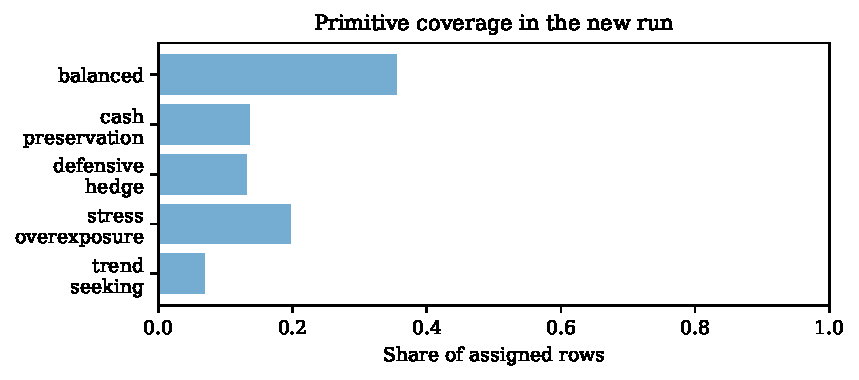
\includegraphics[width=0.82\linewidth]{figures/primitive_coverage.pdf}
\caption{Primitive coverage for the new real-market run.}
\label{fig:primitive-coverage}
\end{figure}
The bars show how often each code appears, not whether it is profitable.

\paragraph{Intervention part.}
The intervention part asks whether the discovered modes are behaviorally specific and whether a narrow edit is safer than rewriting the full controller.

\paragraph{Result 1: Hidden states and hidden actions are control surfaces.}
The short note's result is retained as the design hypothesis: the hidden state and hidden action are potential control surfaces because an edit can be passed through the original action head. In the new run, the hidden-state component is represented by a stable behavior primitive and the hidden-action component by an explicit action adapter. The experiment therefore tests the control-surface logic at the exported action interface rather than claiming access to unexported PPO activations.

\begin{figure}[H]
\centering
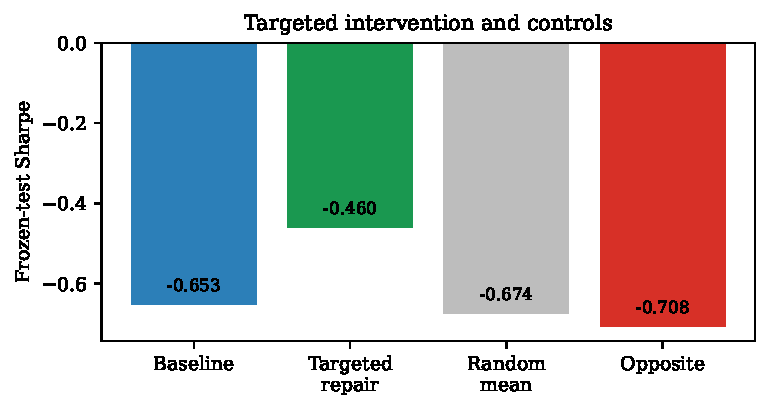
\includegraphics[width=0.78\linewidth]{figures/control_adjusted_effect.pdf}
\caption{Control-surface diagnostic on the new frozen test.}
\label{fig:control-surfaces}
\end{figure}
The targeted adapter and comparison edits produce different gross-return Sharpe values in this window.

\paragraph{Result 2: Best type of intervention.}
The validation selector compares a small set of interventions. It selects the primitive and replacement action jointly and never uses the frozen test for selection. In the current run, primitive 0 is labelled stress overexposure and is mapped to cash preservation. The frozen policy and Q-table remain unchanged.

\begin{figure}[H]
\centering
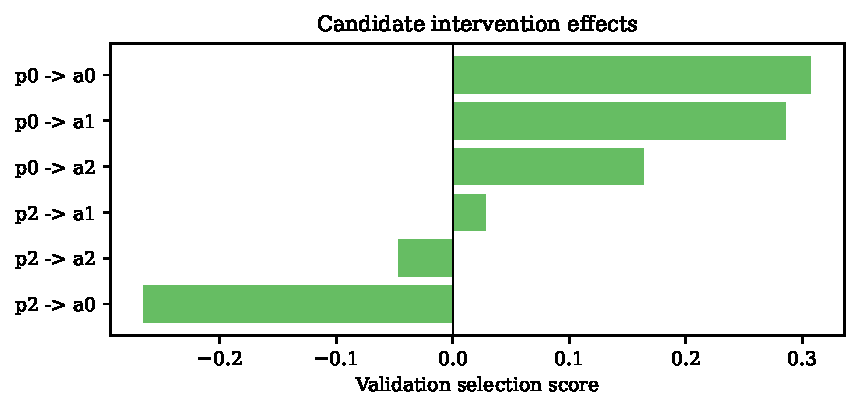
\includegraphics[width=0.80\linewidth]{figures/best_intervention_family.pdf}
\caption{Validation selection scores for candidate primitive-to-action repairs.}
\label{fig:best-intervention}
\end{figure}
The validation score ranks the candidate mappings before the selected mapping is evaluated later.

\begin{table}[H]
\centering
\caption{Intervention questions preserved from the short note and their operational types.}
\label{tab:intervention-types}
\small
\begin{tabular}{@{}p{0.68\linewidth}p{0.20\linewidth}@{}}
\toprule
Question & Type\\
\midrule
If a primitive corresponds to locally harmful behavior, can suppressing it improve out-of-sample counterfactual performance? & Suppression\\
If a primitive corresponds to locally beneficial behavior, can promoting it improve out-of-sample counterfactual performance? & Promotion\\
If the usefulness of a primitive depends on market regime, can we identify the best primitive for each context and use that map as a train-only target for later interventions? & Best-context motivation\\
If a primitive is suboptimal in a given market context, can replacing it with a more context-appropriate primitive improve out-of-sample counterfactual performance? & Replacement\\
If performance degradation is concentrated in a small subset of harmful primitives, can targeted repairs improve out-of-sample counterfactual performance without rewriting the full policy? & Repair\\
\bottomrule
\end{tabular}
\end{table}
Each intervention type asks a different question about whether a behavioral mode can be changed usefully.

\paragraph{Result 3: Hidden state plus hidden action control works better together.}
The combined interface is the practically relevant unit: the primitive identifies a recurring mode and the action adapter specifies the minimal edit. In this run, the combined edit is evaluated against matched-random remappings and an opposite-direction negative control. The targeted repair improves the frozen-test risk profile, but the outer holdout shows that this local gain is not a universal policy improvement.

\begin{figure}[H]
\centering
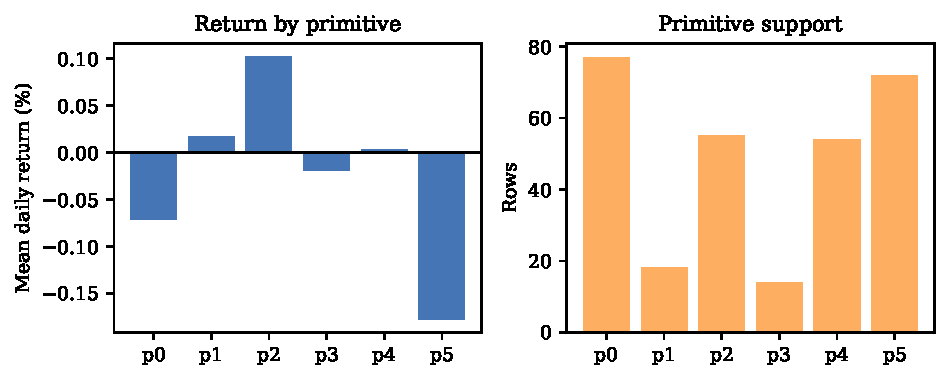
\includegraphics[width=0.90\linewidth]{figures/primitive_return_contribution.pdf}
\caption{Primitive-level return contribution and support on the frozen test.}
\label{fig:primitive-contribution}
\end{figure}
Primitive returns are conditional descriptions of this path, and support indicates how much data backs each value.

\subsubsection{Self-supervised learning references and why they matter here}
The primitive layer is related to several established SSL ideas. VQ-VAE makes a discrete codebook a first-class representation object \cite{oord2017vqvae}; Deep InfoMax maximizes mutual-information objectives between local and global representations \cite{hjelm2019infomax}; SimCLR shows the value of augmentations and contrastive agreement \cite{chen2020simclr}; MoCo uses a momentum-updated dictionary for contrastive representation learning \cite{he2020moco}; and BYOL demonstrates that useful representations can emerge without explicit negative pairs \cite{grill2020byol}. The present financial application is narrower: it uses a compact behavior vocabulary to expose an intervention interface, not to claim that SSL alone produces a trading edge.

\subsection{Controls and evaluation}
The intervention is compared with twenty matched-random remappings that use the same replacement action but a randomly selected non-target primitive. An opposite-direction negative control maps the target primitive to full-equity exposure. The control-adjusted effect is the targeted frozen-test Sharpe minus the mean matched-random Sharpe. Performance claims are reported by split, with both previously inspected evaluation windows treated as historical research comparisons.

\begin{figure}[H]
\centering
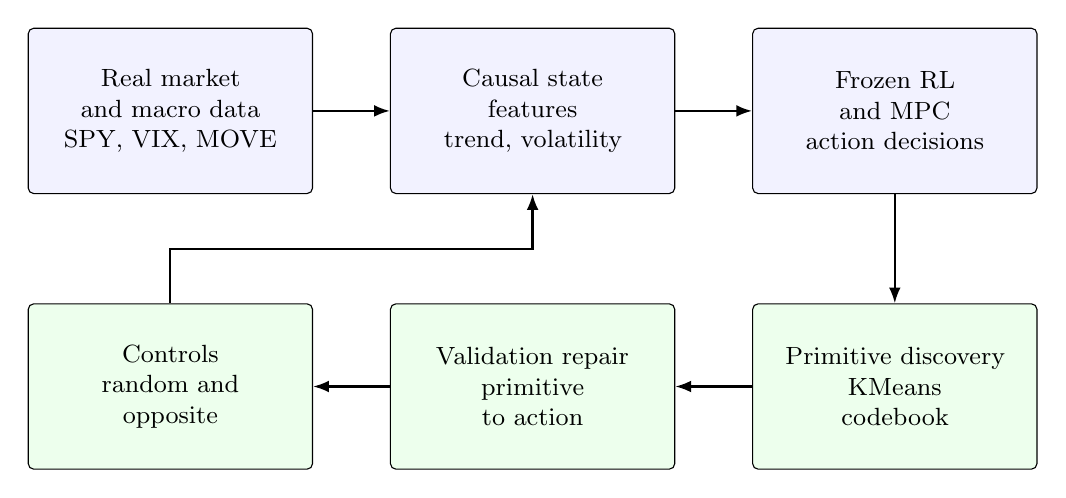
\begin{tikzpicture}[
  box/.style={draw,rounded corners=2pt,align=center,text width=34mm,
    minimum height=21mm,inner sep=3pt,font=\small,fill=blue!5},
  gate/.style={box,fill=green!7},
  arrow/.style={-{Latex[length=2mm]},thick}]
\node[box] (data) at (0,0) {Real market\\and macro data\\SPY, VIX, MOVE};
\node[box] (state) at (4.6,0) {Causal state\\features\\trend, volatility};
\node[box] (controllers) at (9.2,0) {Frozen RL\\and MPC\\action decisions};
\node[gate] (controls) at (0,-3.5) {Controls\\random and\\opposite};
\node[gate] (intervene) at (4.6,-3.5) {Validation repair\\primitive\\to action};
\node[gate] (primitive) at (9.2,-3.5) {Primitive discovery\\KMeans\\codebook};
\draw[arrow] (data.east) -- (state.west);
\draw[arrow] (state.east) -- (controllers.west);
\draw[arrow] (controllers.south) -- (primitive.north);
\draw[arrow] (primitive.west) -- (intervene.east);
\draw[arrow] (intervene.west) -- (controls.east);
% Dedicated corridor: 14 mm clearance from either row of boxes.
\draw[arrow] (controls.north) -- (0,-1.75) -- (4.6,-1.75) -- (state.south);
\end{tikzpicture}
\caption{Reproducible XAI loop; the return arrow follows the open corridor between rows.}
\label{fig:pipeline}
\end{figure}
The loop routes the control comparison back to the feature-based diagnosis without changing the frozen policy.


\section{Software Architecture and Implementation}
The implementation is a single reproducible Python program. It loads the real market files, constructs causal features, fits Q-learning, runs MPC, discovers primitives, and writes machine-readable artifacts. Stage 0 records the data contract and splits. Stage 0.1 records model outputs. Stages 1--3 record primitive discovery and labels. Stage 4 locks the frozen test. Stages 5--6 record the control surface and repair adapter. Stages 7--9 record post-intervention results, controls, and the final verdict.

The remote panel was cross-checked on host \texttt{tsinghua-quant}; the local copy is used for the reported run so that the course submission contains all inputs needed for reproduction. The full stage artifacts are stored in \texttt{artifacts/stage0} through \texttt{artifacts/stage9}.

\section{Data Description and Experimental Design}
The main panel contains daily adjusted prices for SPY, TLT, HYG, and LQD, plus VIX, VIX3M, and MOVE. Derived features include one-day returns, twenty-day SPY momentum and volatility, VIX term structure, HYG minus LQD relative performance, and five-day changes in STLFSI4 and the 10Y--2Y spread. The market data are real US observations from 2010-01-04 through 2026-07-07. The loader merges the latest available FRED/ALFRED vintages by observation date; this is not a point-in-time release reconstruction. Those macro columns are diagnostic and do not enter the tabular policy or the MPC scores.

\begin{table}[H]
\centering
\caption{Time splits and their roles in the experiment.}
\label{tab:splits}
\begin{tabular}{@{}lll@{}}
\toprule
Split & Dates & Purpose\\
\midrule
Train & 2010-01-04 to 2017-12-29 & Q-learning and primitive fit\\
Validation & 2018-01-02 to 2021-12-31 & Repair selection\\
Frozen test & 2022-01-03 to 2023-02-28 & Historical Stage A and Stage C\\
Outer holdout & 2023-03-01 to 2026-07-07 & Exploratory robustness check\\
\bottomrule
\end{tabular}
\end{table}
The dates distinguish fitting, selection, and already-inspected historical evaluation periods.

The saved trajectory column \texttt{ret} contains gross simple portfolio returns. To avoid confusing those returns with the RL reward $r_t$, denote the evaluation returns by $g_t$. For $T$ observations, define
\begin{equation}
\begin{aligned}
 \bar g&=\frac1T\sum_{t=1}^{T}g_t,\qquad
 s_g=\sqrt{\frac{1}{T-1}\sum_{t=1}^{T}(g_t-\bar g)^2},\\
 \mathrm{Sharpe}&=\sqrt{252}\,\frac{\bar g}{s_g},\qquad
 W_t=\prod_{u=1}^{t}(1+g_u),\\
 \mathrm{MaxDD}&=\min_{1\le t\le T}
       \left(\frac{W_t}{\max_{1\le u\le t}W_u}-1\right).
\end{aligned}
\label{eq:metrics}
\end{equation}
Sharpe measures average return relative to volatility, and drawdown measures the largest fall from a previous wealth peak.
Here $T$ counts daily observations; $t$ is the current observation and $u$ a dummy index over earlier ones. $\bar g$ is arithmetic mean daily return; $s_g$ is sample standard deviation, with denominator $T-1$. The square root $\sqrt{252}$ annualizes daily Sharpe under the 252-trading-day convention and a zero risk-free benchmark. $W_t$ is normalized gross wealth starting from 1; the product sign compounds observed returns. The inner maximum is the highest observed wealth up to $t$, the ratio measures retained peak wealth, subtraction of 1 converts it to a signed drawdown, and the outer minimum finds the worst drawdown. The saved implementation starts its peak at the first observed wealth, excluding initial wealth from that maximum. A zero-volatility cash path has undefined Sharpe: the helper's numerical output 0 is displayed as N/A here.

Annualized return is $(W_T/W_0)^{252/T}-1$, where $W_0=1$ and $W_T$ is terminal gross wealth. Turnover is the mean of the successive target changes $\tau_t$, with the first row counted as zero by the metrics helper. Hit rate is the fraction of observations with $g_t>0$; zero-return cash rows do not count as wins. Costs affect the objectives but are not debited from the saved wealth series.

\section{Experimental Results}
\subsection{Stage A: baseline comparison}
\begin{table}[H]
\centering
\caption{Stage A performance before intervention.}
\label{tab:stage-a}
\begin{tabular}{@{}lrrrr@{}}
\toprule
Model & Annual return & Sharpe & Max drawdown & Turnover\\
\midrule
RL validation & 9.72\% & 0.880 & -15.93\% & 24.75\%\\
MPC validation & 2.29\% & 0.316 & -13.22\% & 13.79\%\\
RL frozen test & -11.51\% & -0.653 & -21.71\% & 18.71\%\\
MPC frozen test & 3.05\% & 0.322 & -6.62\% & 7.41\%\\
\bottomrule
\end{tabular}
\end{table}
The ranking between the baseline controllers changes across historical periods.

On validation, RL is more profitable than baseline MPC but trades more and carries greater drawdown. The frozen test reverses the ranking: RL loses 11.51\% annualized with Sharpe $-0.653$, while MPC earns 3.05\% annualized with Sharpe $0.322$ and a much smaller drawdown. This is a direct example of why validation return alone is not an adequate selection criterion in a drifting market.

\subsection{Stage B: diagnosis and repair}
The selected primitive is a stress-overexposure mode. Validation compares stress primitives and replacement actions 0, 1, and 2. Primitive 0 mapped to cash preservation gives the highest validation selection score: Sharpe lift $0.306$ plus a small drawdown-relief term. The frozen policy and Q-table remain unchanged; only the primitive-to-action adapter is edited.

\begin{figure}[H]
\centering
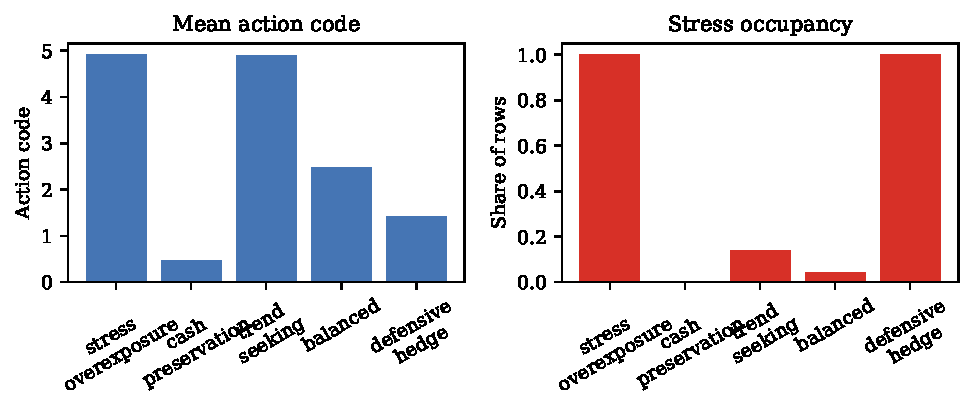
\includegraphics[width=0.92\linewidth]{figures/primitive_profiles.pdf}
\caption{New-market primitive profiles. The codebook is fit on training behavior and assigned forward to validation and test rows.}
\label{fig:primitive-profiles}
\end{figure}
Stress occupancy describes each cluster; numeric action codes are identifiers rather than a calibrated risk scale.

\subsection{Stage C: post-intervention comparison}
\begin{table}[H]
\centering
\caption{Frozen-test Stage C comparison.}
\label{tab:stage-c}
\begin{tabular}{@{}lrrrr@{}}
\toprule
Model & Annual return & Sharpe & Max drawdown & Turnover\\
\midrule
RL frozen test & -11.51\% & -0.653 & -21.71\% & 18.71\%\\
RL repaired frozen test & -6.70\% & -0.460 & -14.95\% & 19.22\%\\
MPC frozen test & 3.05\% & 0.322 & -6.62\% & 7.41\%\\
MPC robust frozen test & 0.27\% & 0.074 & -7.84\% & 7.24\%\\
\bottomrule
\end{tabular}
\end{table}
The targeted RL repair reduces the recorded drawdown, while the state gate does not improve every metric.

The RL repair improves frozen-test Sharpe from $-0.653$ to $-0.460$, changes turnover from 18.71\% to 19.22\%, and improves maximum drawdown from $-21.71\%$ to $-14.95\%$. Annualized return improves from $-11.51\%$ to $-6.70\%$ but remains negative, so this is a risk-control and debugging result rather than evidence of a profitable strategy. The matched-random mean Sharpe is $-0.674$; the control-adjusted lift is $+0.214$. The opposite-direction negative control has Sharpe $-0.708$.

\begin{figure}[H]
\centering
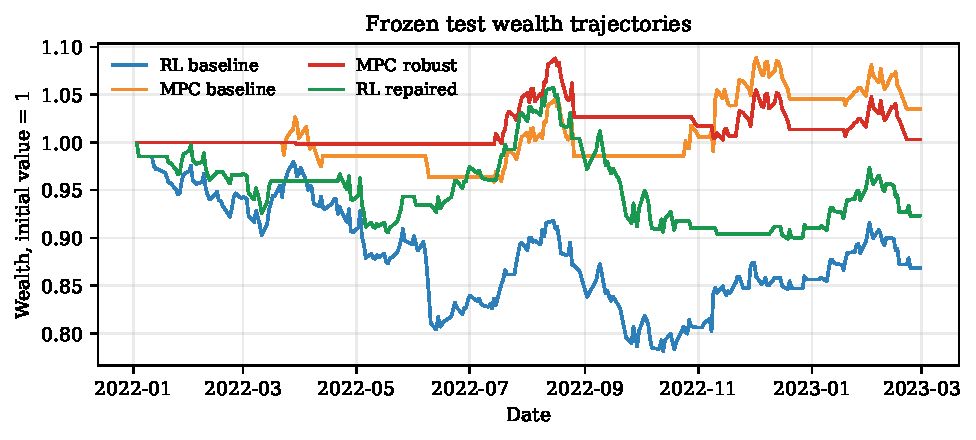
\includegraphics[width=0.92\linewidth]{figures/wealth_stage_A_C.pdf}
\caption{Frozen-test wealth trajectories for Stage A and Stage C.}
\label{fig:wealth}
\end{figure}
The curves show how each recorded gross return path accumulates over the same period.

\begin{figure}[H]
\centering
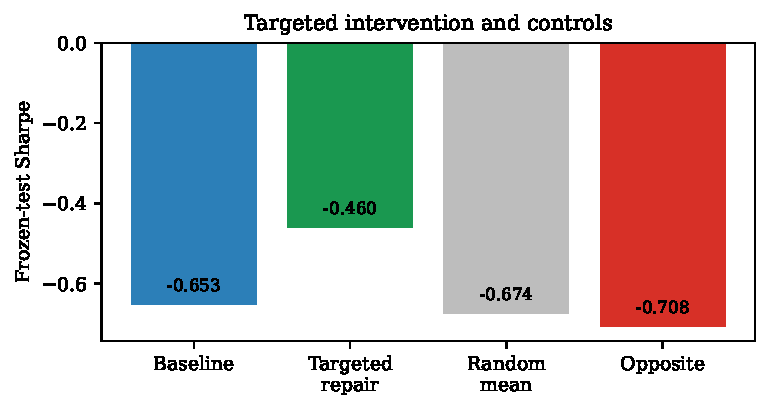
\includegraphics[width=0.78\linewidth]{figures/control_adjusted_effect.pdf}
\caption{Targeted repair compared with matched-random and opposite-direction controls.}
\label{fig:controls}
\end{figure}
Comparison edits help assess specificity, but these controls do not establish statistical significance.

\subsection{Additional MPC experiments: ensemble and minimax robust control}
The two additional controllers use the same six-action grid, horizon $H=5$, risk-aversion coefficient $\lambda=8$, and turnover cost $c=0.0006$ as the baseline. The ensemble combines equally weighted rolling estimators with memory lengths $20$, $60$, and $120$ trading days. The minimax controller evaluates each candidate under all three estimators and retains the worst score before taking the action. No ensemble weight or minimax rule is selected on the frozen test.

\begin{table}[H]
\centering
\caption{Additional MPC experiments and the existing MPC comparators.}
\label{tab:extra-mpc}
\small
\begin{tabular}{@{}llrrrr@{}}
\toprule
Split & Controller & Annual return & Sharpe & Max drawdown & Turnover\\
\midrule
Validation & Baseline & 2.29\% & 0.316 & -13.22\% & 13.79\%\\
Validation & State robust & 13.89\% & 2.246 & -5.90\% & 14.73\%\\
Validation & Ensemble & 2.06\% & 0.283 & -11.76\% & 7.84\%\\
Validation & Minimax robust & 0.29\% & 0.077 & -14.97\% & 7.51\%\\
Frozen test & Baseline & 3.05\% & 0.322 & -6.62\% & 7.41\%\\
Frozen test & State robust & 0.27\% & 0.074 & -7.84\% & 7.24\%\\
Frozen test & Ensemble & -6.37\% & -1.171 & -7.72\% & 4.74\%\\
Frozen test & Minimax robust & 0.00\% & N/A & 0.00\% & 0.00\%\\
Outer holdout & Baseline & 6.06\% & 0.728 & -11.10\% & 12.69\%\\
Outer holdout & State robust & 14.21\% & 1.990 & -7.44\% & 13.88\%\\
Outer holdout & Ensemble & 6.87\% & 0.804 & -7.44\% & 6.12\%\\
Outer holdout & Minimax robust & 3.36\% & 0.495 & -12.00\% & 7.49\%\\
\bottomrule
\end{tabular}
\end{table}
Averaging and worst-case selection yield different exposure choices even on the same action grid.

The ensemble has lower turnover in the later window, but loses on the 2022--2023 window. An audit recomputed all six minimax scores on all 290 historical test rows: cash was the strict winner on 290/290 rows, with a minimum margin of 0.0009 over the best non-cash candidate. The recorded action was 0 and the gross return was zero on every row. The first row uses the initialization moments; subsequent rows use available rolling data. This confirms the plotted horizontal path follows the implemented choice rule rather than a missing data series.

For cash, the three risky weights are zero. After the first transition its expected risky return, variance penalty, and turnover are all zero, whereas every non-cash alternative has a lower worst-model score. The meaning is complete abstention from risk over this window, not successful market timing. The reported wealth stays at 1 because cash earns no interest and the saved returns exclude trading costs. The initial reference action is 2: moving from that target to cash incurs 0.0006 in the score, but the legacy wealth plot does not debit it. Debiting just this one-off penalty would give a flat path at 0.9994 instead. With exactly zero return volatility, economic Sharpe is undefined, even though the old helper stores 0. The outer-window strategy does re-enter risky assets. Ensemble and minimax actions disagree on 14.48\% of the historical test rows.

\paragraph{Takeaway.} The ensemble smooths estimation noise, whereas minimax robust control protects against disagreement by accepting the possibility of an all-cash decision.

\begin{figure}[H]
\centering
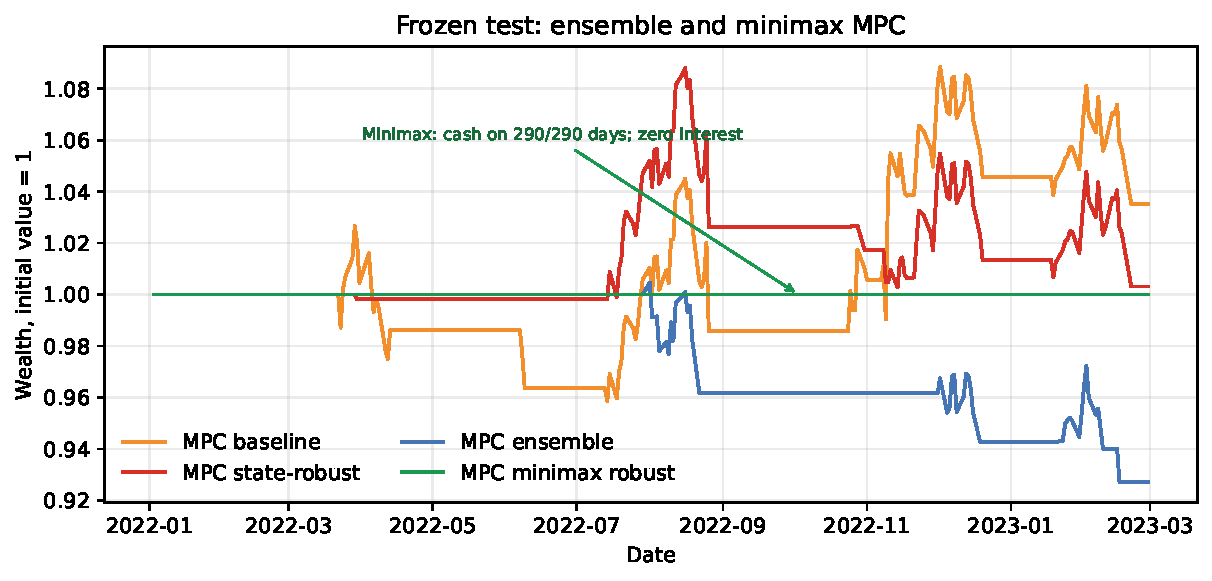
\includegraphics[width=0.92\linewidth]{figures/extra_mpc_frozen_test_wealth.pdf}
\caption{Historical test wealth for the four MPC variants. The flat minimax path is an all-cash, zero-interest, gross-return trajectory, verified over all 290 decisions.}
\label{fig:extra-mpc-wealth}
\end{figure}
The horizontal minimax curve means that this controller took no risky exposure during the entire window.

\begin{figure}[H]
\centering
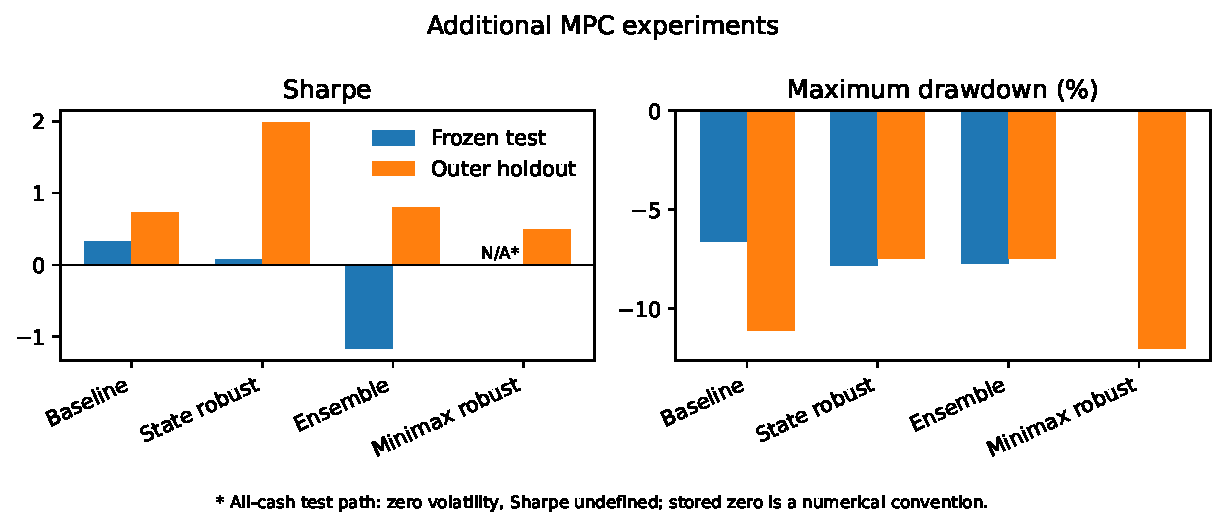
\includegraphics[width=0.90\linewidth]{figures/extra_mpc_comparison.pdf}
\caption{Sharpe and maximum drawdown for the additional MPC experiments on the frozen test and outer holdout.}
\label{fig:extra-mpc-comparison}
\end{figure}
All four controllers are shown; minimax's zero-volatility test Sharpe is marked N/A rather than treated as a measured zero.

\paragraph{Takeaway.} The new graphs separate return-risk behavior from the original state-dependent robust controller and make the minimax conservatism visible.

\subsection{Outer holdout}
\begin{table}[H]
\centering
\caption{Exploratory outer holdout after the frozen test.}
\label{tab:outer}
\begin{tabular}{@{}lrrrr@{}}
\toprule
Model & Annual return & Sharpe & Max drawdown & Turnover\\
\midrule
RL outer holdout & 15.13\% & 1.451 & -10.89\% & 23.25\%\\
RL repaired outer holdout & 6.69\% & 0.800 & -10.89\% & 24.91\%\\
MPC outer holdout & 6.06\% & 0.728 & -11.10\% & 12.69\%\\
MPC robust outer holdout & 14.21\% & 1.990 & -7.44\% & 13.88\%\\
MPC ensemble outer holdout & 6.87\% & 0.804 & -7.44\% & 6.12\%\\
MPC minimax outer holdout & 3.36\% & 0.495 & -12.00\% & 7.49\%\\
\bottomrule
\end{tabular}
\end{table}
The later period reverses some earlier gains, so no controller dominates every historical window.

The outer holdout changes the interpretation. Robust MPC reaches Sharpe $1.990$ with maximum drawdown $-7.44\%$, whereas baseline MPC reaches Sharpe $0.728$ with maximum drawdown $-11.10\%$. The RL repair does not generalize as a universal improvement: repaired RL has Sharpe $0.800$ versus $1.451$ for baseline RL. This is the type of drift alert that the XAI layer is intended to expose.

\section{Conclusion}
The before--after experiment demonstrates a practical XAI workflow for sequential portfolio decisions. MPC provides a readable controller and strong drawdown protection under the reported stress split. RL provides an adaptable challenger but is vulnerable to regime drift. The ensemble and minimax MPC experiments show two different responses to model uncertainty: averaging lowers turnover, while worst-case scoring can refuse risky exposure. A primitive-based intervention selected on validation improves frozen-test RL behavior relative to matched-random edits, yet the outer holdout shows that the repair is local rather than universal. The defensible conclusion is methodological: explanations are useful when they identify an editable behavior, specify a low-dose intervention, and survive negative controls.

\begin{thebibliography}{99}
\bibitem{oord2017vqvae}
A. van den Oord, O. Vinyals, and K. Kavukcuoglu,
``Neural discrete representation learning,'' in \emph{Advances in Neural Information Processing Systems}, 2017.

\bibitem{hjelm2019infomax}
R. D. Hjelm et al.,
``Learning deep representations by mutual information estimation and maximization,'' in \emph{International Conference on Learning Representations}, 2019.

\bibitem{chen2020simclr}
T. Chen, S. Kornblith, M. Norouzi, and G. Hinton,
``A simple framework for contrastive learning of visual representations,'' in \emph{International Conference on Machine Learning}, 2020.

\bibitem{he2020moco}
K. He, H. Fan, Y. Wu, S. Xie, and R. Girshick,
``Momentum contrast for unsupervised visual representation learning,'' in \emph{Proceedings of the IEEE/CVF Conference on Computer Vision and Pattern Recognition}, 2020.

\bibitem{grill2020byol}
J.-B. Grill et al.,
``Bootstrap your own latent: A new approach to self-supervised learning,'' in \emph{Advances in Neural Information Processing Systems}, 2020.

\bibitem{milani2024xrl}
S. Milani, N. Topin, M. Veloso, and F. Fang,
``Explainable reinforcement learning: A survey and comparative review,'' \emph{ACM Computing Surveys}, vol. 56, no. 7, 2024.

\bibitem{atrey2020counterfactual}
A. Atrey, K. Clary, and D. Jensen,
``Exploratory not explanatory: Counterfactual analysis of saliency maps for deep reinforcement learning,'' in \emph{International Conference on Learning Representations}, 2020.

\bibitem{bailey2014dsr}
D. H. Bailey and M. Lopez de Prado,
``The deflated Sharpe ratio: Correcting for selection bias, backtest overfitting and non-normality,'' \emph{Journal of Portfolio Management}, vol. 40, no. 5, pp. 94--107, 2014.

\bibitem{bates1969combination}
J. M. Bates and C. W. J. Granger,
``The combination of forecasts,'' \emph{Journal of the Operational Research Society}, vol. 20, no. 4, pp. 451--468, 1969, doi: 10.1057/jors.1969.103.

\bibitem{timmermann2006forecast}
A. Timmermann,
``Forecast combinations,'' in \emph{Handbook of Economic Forecasting}, vol. 1, 2006, pp. 135--196, doi: 10.1016/S1574-0706(05)01004-9.

\bibitem{ledoit2004honey}
O. Ledoit and M. Wolf,
``Honey, I shrunk the sample covariance matrix,'' \emph{Journal of Multivariate Analysis}, vol. 88, pp. 365--411, 2004, doi: 10.1016/S0047-259X(03)00096-4.

\bibitem{riskmetrics1996}
J. P. Morgan/Reuters,
\emph{RiskMetrics Technical Document}, fourth edition, 1996.

\bibitem{mayne2000constrained}
D. Q. Mayne, J. B. Rawlings, C. V. Rao, and P. O. M. Scokaert,
``Constrained model predictive control: Stability and optimality,'' \emph{Automatica}, vol. 36, no. 6, pp. 789--814, 2000, doi: 10.1016/S0005-1098(99)00214-9.

\bibitem{lobo2000worstcase}
M. Lobo and S. Boyd,
``The worst-case risk of a portfolio,'' Stanford University technical report, 2000.

\bibitem{wang2004robust}
Y. J. Wang and J. B. Rawlings,
``A new robust model predictive control method I: Theory and computation,'' \emph{Journal of Process Control}, vol. 14, no. 3, pp. 231--247, 2004, doi: 10.1016/S0959-1524(02)00133-6.

\bibitem{li2022portfolio-mpc}
X. Li, A. S. Uysal, and J. M. Mulvey,
``Multi-period portfolio optimization using model predictive control with mean-variance and risk parity frameworks,'' \emph{European Journal of Operational Research}, vol. 299, no. 3, pp. 1158--1176, 2022, doi: 10.1016/j.ejor.2021.09.027.
\end{thebibliography}

\end{document}

